\section{Generating Mass and Position for Cluster Particles}
\label{Method:GeneratingPosMassVel}
When considering the time evolution of an $N$-particle star cluster, in which the mass and position of each single particle is not known from a catalogue or of special significance, it is inappropriate to hard code the values for each single particle. 
Instead, it is an advantage to use probability distribution functions to generate random positions and masses for each of the particles. 
It is decided that the mass of the $N$ particles in the cluster should follow a Gaussian distribution around ten solar masses with a standard deviation of one solar mass.
For the position, it is decided that the density of particle initially is uniform in a sphere with a radius of twenty solar masses.
The is, however, not equivalent to saying that the particles are uniformly distributed in the Cartesian coordinates $x$, $y$ and $z$ and neither in the spherical coordinates $r$, $\phi$ and $\theta$, which complicates the problem a bit.
The sections below present the functions for generating random masses an positions of $N$ particles with the desired distributions. 
Each of the functions are tested for a system with $N=100,000$.

\subsection{Gaussian Distributed Mass}
\fxnote{we should probably have a ref. here}

Pseudo-random numbers, corresponding to masses, randomly distributed by a Gaussian distribution is generated following the Box-Muller transform. 
The basic form of the Box-Muller transform gives
\begin{align*}
	X_1 = \sqrt{-2ln(V_1)}sin(2V_2)=Rcos(\theta)
	\\
	X_2 = \sqrt{-2ln(V_1)}cos(2V_2)=Rsin(\theta)
\end{align*}
where $R ^2 = -2ln(V_1)$ and $\theta =2V_1$.
$X_1$ and $X_2$ are random numbers distributed according to a Gaussian distribution of mean 0 and variance 1.
In polar form the above two equations becomes
\begin{align*}
	X_1 = 
	%\sqrt{-2ln(V_1)}sin(2V_2)=\sqrt{-2ln S}  u/\sqrt{s} = 
	u \sqrt{\frac{-2 ln(s)}{s}}
	\\
	X_2 = 
	%\sqrt{-2ln(V_1)}cos(2V_2)=\sqrt{-2ln S}  v/\sqrt{s} = 
	v \sqrt{\frac{-2 ln(s)}{s}}
\end{align*}
where $s = R^2 = u^2 + v^2$. \fxnote{how the hell??}
Here $u$ and $v$ are uniformly distributed in the interval [-1,1] and points only within the unit circle is admitted (see \figref{fig:Gaussian_mass_generation_ill}). 
Therefore, only those pairs of $u$ and $v$ which gives a value for $s$ in the interval (0,1) is considered. 
Value of $s$ is similar to that of $V_1$ and $\theta/2\pi$ is similar to that of $V_2$ in the basic form.
\begin{figure}[H]
\centering
	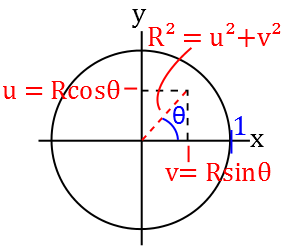
\includegraphics[width=0.4\linewidth]{Figures/Gaussian_mass_generation_ill.png}
\caption{
???
}
\label{fig:Gaussian_mass_generation_ill}
\end{figure}
The lines of code below shows the implementation of the generation of masses normally distributed with a mean of $10\text{M}_{\odot}$ and a standard deviation of $1\text{M}_{\odot}$.
\begin{lstlisting}
void gaussian_mass_generator(vec (&mass), int number_of_particles)
{
  srand(time(NULL));
  for (int i = 0; i < number_of_particles; i++)
  {
  static int iset = 0;
  static double gset;
  double fac, rsq, v1, v2;
    do{
	//generate two random numbers uniformly distributed in the interval [-1,1]   
      v1 = 2.*((double) rand() / (RAND_MAX)) -1.0;
      v2 = 2.*((double) rand() / (RAND_MAX)) -1.0;
      //Radius of the numbers (within the unit circle) squared
      rsq = v1*v1+v2*v2;
    } while (rsq >= 1.0 || rsq == 0.);
    //computing the gaussian distributed numbers
    fac = sqrt(-2.*log(rsq)/rsq);
    gset = v1*fac;
    iset = 1;
    mass(i) = v2*fac;
    mass(i) += 10;
  }
}
\end{lstlisting}
In the function \textit{gaussian\_ mass\_ generator}, v1 and v2 are random numbers uniformly distributed in the interval [-1,1]. $rsq = v1^2 + v2^2$  corresponds to $s = R ^2 = u^2 + v^2$. 
Using the do-while loop only those pairs of v1 and v2 that produces an s equal to 0 or greater than or equal to 1 is generated so that the points are inside unit circle.  Variable gset  correspond to X1.

To test whether the generated masses are actually normally distributed around $10\text{M}_{\odot}$ with a standard deviation of $1\text{M}_{\odot}$, 100,000 masses are generated, by the presented code, and plotted in a histogram below. 
\begin{figure}[H]
\centering
	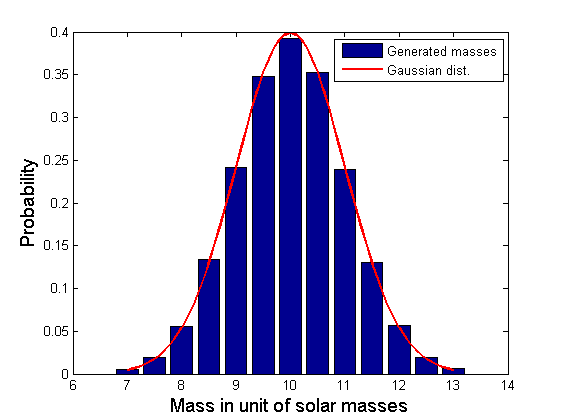
\includegraphics[width=0.7\linewidth]{Figures/random_mass_test.png}
\caption{
Histogram of the mass of 100,000 particles generated by the c++ code introduced above together with a Gaussian distribution of mean $10 \text{R}_{\odot}$ and standard deviation $1 \text{R}_{\odot}$ generated in MatLab using the \textit{normpdf} function. 
}
\label{fig:GaussianGeneratedMass}
\end{figure}

\subsection{Uniformly Distributed Position}
To generate positions uniformly distributed inside a sphere of radius $R_0$, random numbers generated using the \textit{rand} function in c++ are used and converted into coordinates of uniformly distributed particles within the sphere. 
In order to get a uniform density of particles three variables $v$, $w$ and $u$ corresponding to random numbers uniformly distributed between 0 and 1 are introduced.
The spherical coordinates $\theta$, $\phi$ and $r$ are, according to \cite{AddNotesAstroUniDist}, then linked to these variables using the equation
\begin{align*}
	&\theta = cos^{-1}(1-2v)
	\\
	&\phi = 2\pi w
	\\	
	&r = R_0 (u)^{1/3}
\end{align*}                                            
The following equations are then used to get back to the Cartesian coordinate system.
\begin{align*}
	&x= rsin(\theta)cos(\phi)
	\\
    &y = r sin(\theta) sin(\phi)
    \\
    &z = r cos(\theta)
\end{align*}
After performing these steps, a uniform distribution of $N$ particles within a sphere of radius $R_0$ is achieved.
Below, the code for generating this uniform distribution within a sphere of radius $R_0 = 20 \text{ly}$ is introduced.
\begin{lstlisting}
void uniform_pos_generator(mat (&position), int N)
{
double pi=3.14159, c = 2*pi, R = 20;
vec phi(N), r(N), theta(N), x(N), y(N), v(N);

srand(time(NULL));

for (int i=0;i<N;i++){

        x(i) = ((double) rand() / (RAND_MAX)); //random numbers generated in the interval(0,1)
        y(i) = ((double) rand() / (RAND_MAX));
        v(i) = ((double) rand() / (RAND_MAX));
   }
for (int i=0;i<N;i++){
        phi(i)=c*x(i);
        r(i)=R*pow(y(i),1.0/3.0);
        theta(i)=acos(1.0-2.0*v(i));
        position(i,0)=r(i)*sin(theta(i))*cos(phi(i));
        position(i,1)=r(i)*sin(theta(i))*sin(phi(i));
        position(i,2)= r(i)*cos(theta(i));
   }
}
\end{lstlisting}
To test whether the generated positions within the sphere of radius $20$ ly, the density of particles in the cross-sectional area of each $x$-value is determined and plotted as a histogram in \figref{fig:UniformlyGeneratedPos} for $100,000$ particles with position generated by the introduced lines of code.  
The density of particles in the cross-sectional area of each $x$-value is found by dividing the total number of particles with that $x$-value with the cross-sectional area of the sphere in that $x$-value (see \figref{fig:Cross_sectional_area}).
\begin{figure}[H]
\centering
	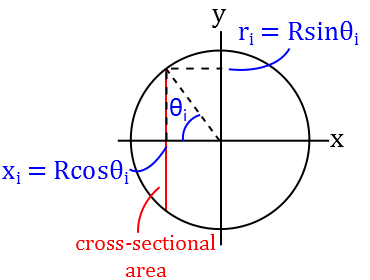
\includegraphics[width=0.4\linewidth]{Figures/Cross_sectional_area.png}
\caption{
Two-dimensional illustration of the three-dimensional problem of determining the density of particles in each $x$-value.
}
\label{fig:Cross_sectional_area}
\end{figure}
The cross-sectional area of the sphere in a specific area is found from a little trigonometry, by first considering that the radius of the circle that makes of the cross-sectional area in a point $x_i$ is given by $r_i = 20sin\theta_i$ ly.  
This yields that the area $A_i$ of the cross-sectional area, in ly, is given as
\begin{align}
	A_i = 400\pi sin^2 \theta_i =  400\pi (1 - cos^2 \theta)
\end{align}
in which the last equal sign stems from $1 = cos^2 \theta + sin^2 \theta$.
But $x_i = 20 cos \theta_i$ ly, giving
\begin{align}
	A_i = \pi (400 - x_i^2)
\end{align}
\begin{figure}[H]
\centering
	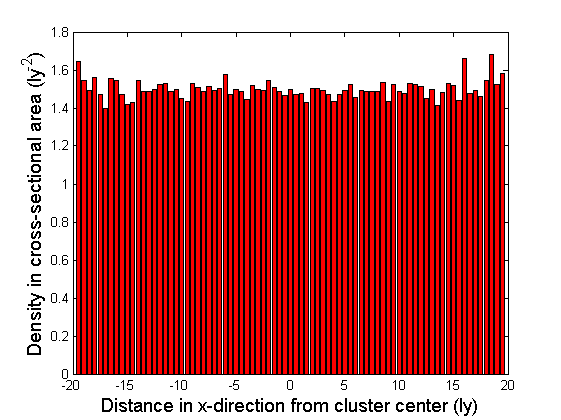
\includegraphics[width=0.7\linewidth]{Figures/random_uniform_position_test.png}
\caption{
Histogram of density of 100,000 particles with position generated by the code introduced in \fxnote{where??} as a function of the $x$-coordinate of the particles. The histogram is made with bins in the interval [$-19.5;19.5$] and a bin-size of $0.5$. The distance $x = \pm 20$ from the cluster center is not considered, since the cross-sectional area in that point is zero.
}
\label{fig:UniformlyGeneratedPos}
\end{figure}